% ── Rozwiązanie: Huffman -- instancja 2 ──────────────────────────
\subsection{Algorytm Huffmana -- instancja 2}

Dane: kolejka startowa $(g, 2),\ (o, 3),\ (k, 6),\ (m, 8),\ (l, 11),\ (u, 14),\ (e, 20)$,
sumaryczna częstość $64$. W~każdej z~$n - 1 = 6$ iteracji łączymy dwa korzenie
o~\emph{najmniejszej} częstości (mniejszy jako lewe dziecko, krawędź $0$; remisy
wg~kolejności w~kolejce), wstawiając nowy wierzchołek z~powrotem. Style drzew
i~makro \texttt{\textbackslash huffstep} przejęte z~instancji~1.

\tikzset{
	htree/.style={
			level distance=0.95cm,
			level 1/.style={sibling distance=3.4cm},
			level 2/.style={sibling distance=1.9cm},
			level 3/.style={sibling distance=1.2cm},
			level 4/.style={sibling distance=1.0cm},
			every node/.style={circle, draw, minimum size=0.7cm, inner sep=0pt, font=\footnotesize, align=center},
			elabel left/.style={draw=none, font=\scriptsize, inner sep=1pt, midway, sloped, above},
			elabel right/.style={draw=none, font=\scriptsize, inner sep=1pt, midway, sloped, above},
		}
}

\huffstep{%
	\textbf{1.} Łączymy $g$ i~$o$. \\
	Zostają: $(5), (k, 6), (m, 8), (l, 11), (u, 14), (e, 20)$.
}{%
	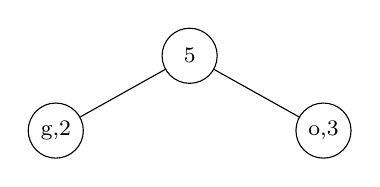
\begin{tikzpicture}[htree]
		\node {5}
		child { node {g,2} }
		child { node {o,3} };
	\end{tikzpicture}
}

\huffstep{%
	\textbf{2.} Łączymy $5$ i~$k$. \\
	Zostają: $(m, 8), (11), (l, 11), (u, 14), (e, 20)$.
}{%
	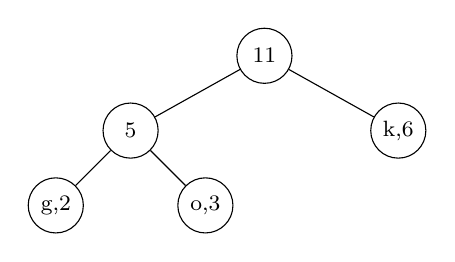
\begin{tikzpicture}[htree]
		\node {11}
		child { node {5}
				child { node {g,2} }
				child { node {o,3} }
			}
		child { node {k,6} };
	\end{tikzpicture}
}

\huffstep{%
	\textbf{3.} Łączymy $m$ i~$l$. \\
	Zostają: $(11), (u, 14), (19), (e, 20)$.
}{%
	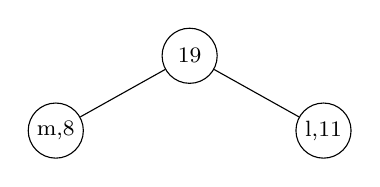
\begin{tikzpicture}[htree]
		\node {19}
		child { node {m,8} }
		child { node {l,11} };
	\end{tikzpicture}
}

\huffstep{%
	\textbf{4.} Łączymy $11$ i~$u$. \\
	Zostają: $(19), (e, 20), (25)$.
}{%
	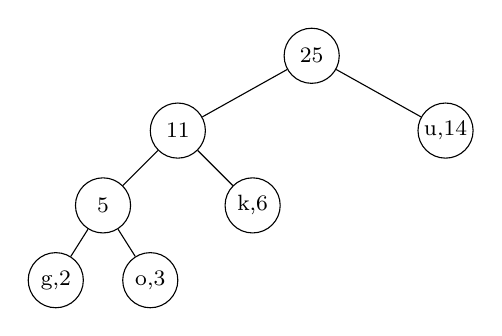
\begin{tikzpicture}[htree]
		\node {25}
		child { node {11}
				child { node {5}
						child { node {g,2} }
						child { node {o,3} }
					}
				child { node {k,6} }
			}
		child { node {u,14} };
	\end{tikzpicture}
}

\huffstep{%
	\textbf{5.} Łączymy $19$ i~$e$. \\
	Zostają: $(25), (39)$.
}{%
	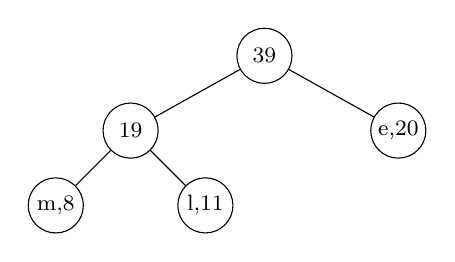
\begin{tikzpicture}[htree]
		\node {39}
		child { node {19}
				child { node {m,8} }
				child { node {l,11} }
			}
		child { node {e,20} };
	\end{tikzpicture}
}

\huffstep{%
	\textbf{6.} Łączymy $25$ i~$39$. \\
	(ostateczne drzewo kodów)
}{%
	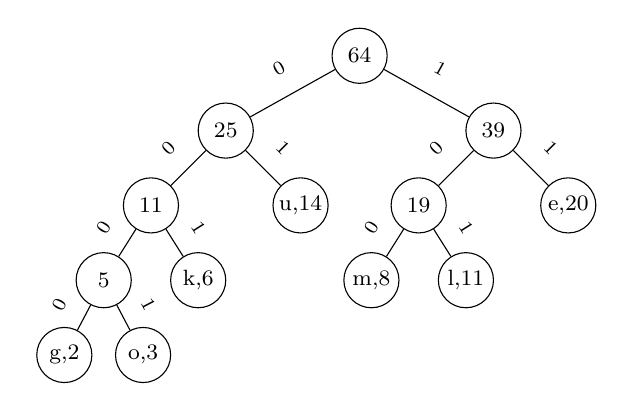
\begin{tikzpicture}[htree]
		\node {64}
		child { node {25}
				child { node {11}
						child { node {5}
								child { node {g,2} edge from parent node[elabel left] {0} }
								child { node {o,3} edge from parent node[elabel right] {1} }
								edge from parent node[elabel left] {0}
							}
						child { node {k,6} edge from parent node[elabel right] {1} }
						edge from parent node[elabel left] {0}
					}
				child { node {u,14} edge from parent node[elabel right] {1} }
				edge from parent node[elabel left] {0}
			}
		child { node {39}
				child { node {19}
						child { node {m,8} edge from parent node[elabel left] {0} }
						child { node {l,11} edge from parent node[elabel right] {1} }
						edge from parent node[elabel left] {0}
					}
				child { node {e,20} edge from parent node[elabel right] {1} }
				edge from parent node[elabel right] {1}
			};
	\end{tikzpicture}
}

Odczytany kod z~drzewa w~kroku 6:
\begin{flalign*}
	u & \implies 01   &  & \\
	e & \implies 11   &  & \\
	k & \implies 001  &  & \\
	m & \implies 100  &  & \\
	l & \implies 101  &  & \\
	g & \implies 0000 &  & \\
	o & \implies 0001 &  &
\end{flalign*}

\paragraph{Liczba bitów.}
\[
	\boxed{B(T) = 2\cdot 4 + 3\cdot 4 + 6\cdot 3 + 8\cdot 3 + 11\cdot 3 + 14\cdot 2 + 20\cdot 2 = 163 \text{ bitów}}
\]
(wobec $64 \cdot 3 = 192$ bitów przy kodzie stałej długości po $3$ bity na znak).
